\chapter{Data Analysis}
In the analysis of experimental data, the primary goals are to extract the $2n$ removal cross section in the ${}^{17}\text{B} \to {}^{15}\text{B} + 2n$ reaction and to obtain the Relative energy spectrum. To achieve this, I will describe the procedure of identifying the secondary beam of ${}^{17}$B, and \textcolor{red}{selecting events involving the fragment ${}^{15}$B and two neutrons. Particular emphasis is placed on the process of selecting two-neutron events and the rejection of cross-talk.} The flow of the Data Analysis is as follows.

\begin{center}
    \begin{enumerate}[noitemsep]
        \item Select the event containing ${}^{17}$B beam by beam PID
        \item Select the event containing ${}^{15}$B fragment by fragment PID
        \item Select the event containing two neutron by cross-talk analysis
        \item Extract the 2n removal cross section of the ${}^{17}\text{B} \to {}^{15}\text{B} + 2n$ reaction
        \item Reconstruct Invariant Mass at target and obtain the Relative energy spectrum 
    \end{enumerate}
\end{center}

\section{Analysis of the Secondary Beam}
The primary beam was generated by the SRC, RIBF. By accelerating ${}^{48}$Ca to 345 MeV/u and bombarding it on a thick Be target (30mm), a secondary beam was produced. The characteristics of the primary beam were as follows.
    \begin{table}[ht]
        \centering 
            \begin{tabular}[ht]{c|c|c|c}
                \hline
                Primary Beam & Beam Energy & Beam Intensity & Primary Target  \\
                \hline
                ${}^{48}$Ca & 345 MeV/u & 210 pnA & Be (30mm)\\
                \hline    
            \end{tabular}
        \caption[Short]{Information of Primary Beam}
    \end{table}
\indent The collision between the initial beam and the target created the secondary beam, including not only the experiment's purpose isotope, ${}^{19}$B, but also other neighboring isotopes. The main isotope used in this research is ${}^{17}$B, which needed to be separated and identified through the BigRIPS separator. The identification of the ${}^{17}$B secondary beam was performed using the TOF-B$\rho$-$\Delta$E method. The identified ${}^{17}$B was then transferred to SAMURAI, where it underwent Coulomb Dissociation, the main objective of this research. Three different targets were used: C, Pb, and Empty. The details for ${}^{17}$B with each target were as follows.
    \begin{table}[ht]
        \centering
        \begin{tabular}[ht]{c|c|c}
            \hline
            isotope & Target & Average Energy at Target \\
            \hline
            \hline
            & C (1.789 g/cm2)  & 270 MeV/u\\
            ${}^{17}$B & Empty  & 275 MeV/u\\
            & Pb (3.255 g/cm2) & 270 MeV/u\\
            \hline    
        \end{tabular}
        \caption[short]{Information of Secondary Beam}
    \end{table}

\subsection{Analysis of Time of Flight}
The time-of-flight (TOF) is calculated using the time difference between two plastic scintillators. Three plastic scintillators are used for this TOF calculation. One is located at F7 and the other two, called SBT1 and SBT2, are at F13. The TOF between F7 and F13 is defined as following.
    \begin{align}
        \text{TOF}_{\text{F7-F13}} = \frac{t_{\text{SBT1}} + t_{\text{SBT2}}}{2} - t_{\text{F7}} + \Delta t_{offset}
    \end{align}
$\Delta t_{offset}$ is the offset used to correct for the difference between the actual measured $\text{TOF}_{\text{F7-F13}}$ and the TOF value calculated by considering the material between F7 and F13. For the calculation, runs with the f5 slit narrowed to $\pm$ 1mm (run number 428,429,431) are used,for the mono-energetic isotopes. The calculated $\text{TOF}_{\text{F7-F13}}$ value is 192.333 ns, and the corresponding $\Delta t_{offset}$ value is 172.025 ns. \textcolor{red}{tof 분해능 추가}

\subsection{Analysis of Magnetic Rigidity}
Magnetic Rigidity $B\rho$ is derived by Beam Projection Chamber (BPC) located at dispersive focal plane (F5). The x position of a beam passing through F5 is measured by BPC, and the $B\rho$ is calculated using the following equation.
    \begin{align}
        B\rho = (1+\frac{x}{D}) B\rho_{0} 
    \end{align}
with the rigidity of the central trajectory $B\rho_{0}$, 8.78 Tm, and  momentum dispersion $D$, 3300 cm/$\%$. \textcolor{red}{The position resolution of BPC is ooo from wire spacing 4 mm.} \textcolor{red}{Brho의 분해능 추가}

\subsection{Analysis of Energy Loss}
The energy loss $\Delta$E is measured in the Ionize Chamber for Beam (ICB). The correlation between $\Delta$E and Z can be obtained according to the simplified Bethe-Bloch's Energy loss formula as follows. In this formula, the\textit{density effect} correction $\delta$ or \textit{shell} correction $C$ is skipped.
    \begin{align}
        \frac{dE}{dx} = 2\pi N_{a} r_{e}^{2} m_{e} c^{2} \rho_{\text{P10}} 
        \bigg( \frac{Z_{\text{P10}}}{A_{\text{P10}}} \bigg) \bigg( \frac{Z^{2}}{\beta^{2}} \bigg) 
        \left[ \ln \frac{2m_{e}c^{2}\beta^{2}\gamma^{2}}{I_{\text{P10}}} - \beta^{2}  \right]
    \end{align}
with
    \begin{align}
        2 \pi N_{a} r_{e}^{2} m_{e} c^{2} \rho_{\text{P10}} = 0.307075 \text{ MeV cm}^{2} \text{g}^{-1} 
    \end{align}
    \begin{adjustwidth}{1cm}{}
        $N_{a}$ : Avogadro's number = 6.022 $\times$ 10$^{23}$\\
        $r_{e}$ : classical electron radius = 2.817 $\times$ 10$^{-13}$ cm\\ 
        $m_{e}$ : electron mass = 0.511 MeV/c$^{2}$\\
        $\rho_{\text{P10}}$ : density of the P10 gas = 1.84 $\times$ 10$^{-3}$ g/cm$^{3}$\\
        $Z_{\text{P10}}$ : effective atomic number of the P10 gas\\
        $A_{\text{P10}}$ : effective mass number of the P10 gas\\
        $I_{\text{P10}}$ : mean excitation energy of the P10 gas\\ 
        $\beta$ = $v / c$ of the beam particle\\
        $\gamma$ = $1 / \sqrt{1-\beta^{2}}$
    \end{adjustwidth}
\vspace{2mm}Because of the P10 gas is compound of 90$\%$ Ar and 10$\%$ CH$_{4}$, the mean excitation energy $I_{\text{P10}}$ is calculated as follows. The detail of the calculation of I for compound is described in the Appendix A.

\subsection{Beam Particle Identification}
Secondary beam particles are identified using the TOF-B$\rho$-$\Delta$E method. A/Z and Z is driven by the following equation.
\begin{align}
    \beta_{\text{TOF}} &= L(\text{F7-F13}) / ( {\text{TOF}}_{\text{F7-F13}} \times c )\\
    \beta_{\text{F5}} &= f(\text{TOF}_{\text{F7-F13}})\\
    A/Z &= c B\rho_{\text{F5}} \gamma_{\text{F5}} / m_u \beta_{\text{F5}}
\end{align}
    $\beta_{\text{F5}}$ is polynomial function of 
\begin{align}
    Z = \beta_{\text{TOF}} \sqrt{\Delta E_{\text{ICB}} / ( 0.307075 \times \Delta x \times (Z_{\text{P10}} / A_{\text{P10}} ) \ln(2m_{e}c^{2}\beta^{2}\gamma^{2}/ I_{\text{P10}} - \beta^{2}) )}
\end{align}
$\Delta E_{\text{ICB}}$ is total energy loss at ICB and $\Delta x$ is the thickness of ICB. 
% The travel distance between ICB is calculated (51-0.0262)*0.9*0.0016608 + (51-0.0262)*0.1*0.000667 length*probability*volume density
Figure 4.1 shows the histogram of particle identification of the secondary beam with x-axis as A/Z and y-axis as Z. 
\begin{table}[h]
    \centering
    \begin{tabular}{cccc}
        \hline
        Secondary Beam & Pb target & C target & Empty target\\             
        \hline \hline
        ${}^{19}$B &  2&3  &4  \\
        ${}^{17}$B &  &  &  \\
        ${}^{20}$C &  &  &  \\
        \hline
    \end{tabular}
    \caption{statistic of Secondary Beam}
\end{table}

\begin{figure}[t]
    \centering
    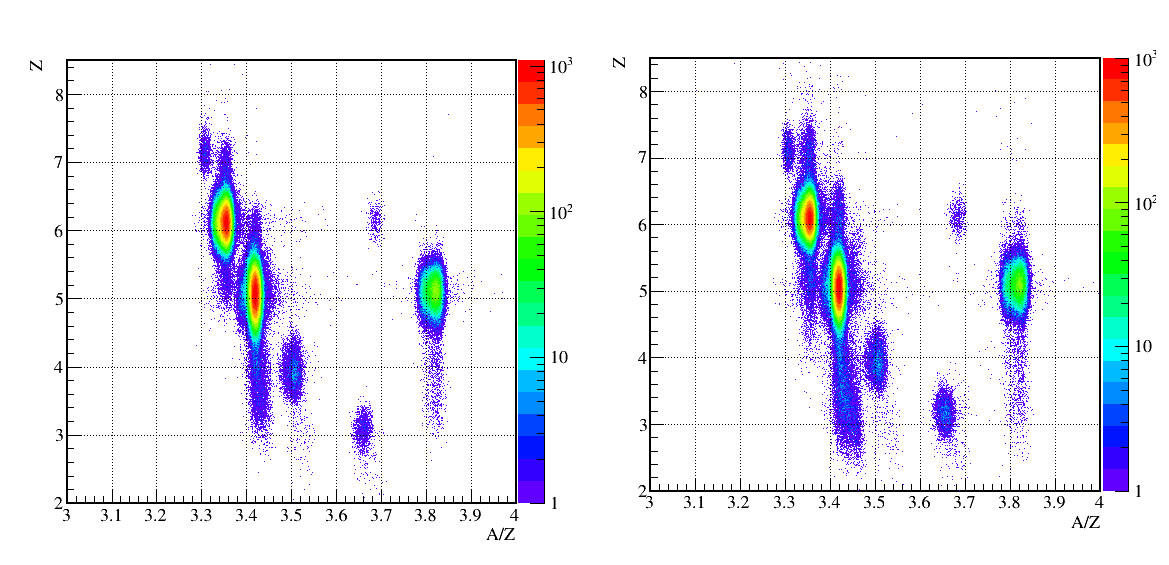
\includegraphics[width=14cm]{chapter4/beampid.png}
    \caption{Beam Particle Identification for Pb target (left) and C target (right)}
    \label{Beam Particle Identification}
\end{figure}

Following table shows each particle's statistic and Intensity

\clearpage
%----------------------------------------------------------------------------------------------------
\section{Beam Profile at Target}
The beam profile at the target can be determined using two drift chambers, BDC1 and BDC2, located upstream of the target. BDC1 and BDC2 are Ionized Drift Chambers that allow for the determination of a particle's trajectory through reconstruction of the hit positions on each layer. By using this feature, the incident position and angle at the each BDC can be determined, and these are then extrapolated to find the incident position and angle at the target.

\subsection{BDC Calibration}

\subsubsection{TDC Distribution}
The timing information of the BDC is obtained using the TDC. And using this information, we can calculate the drift distance
This TDC distribution is obtained from run 431 which is f5 slit is

\begin{table}[h]
    \centering
    \begin{tabular}{c|cc}
        \hline
        &$t_{min}$ [ch]&$t_{max}$ [ch]\\
        \hline
        BDC1&600&800\\
        BDC2&600&800\\        
        \hline
    \end{tabular}
    \caption[short]{TDC window of BDC1 and BDC2}
\end{table}

\begin{figure}
    \centering
    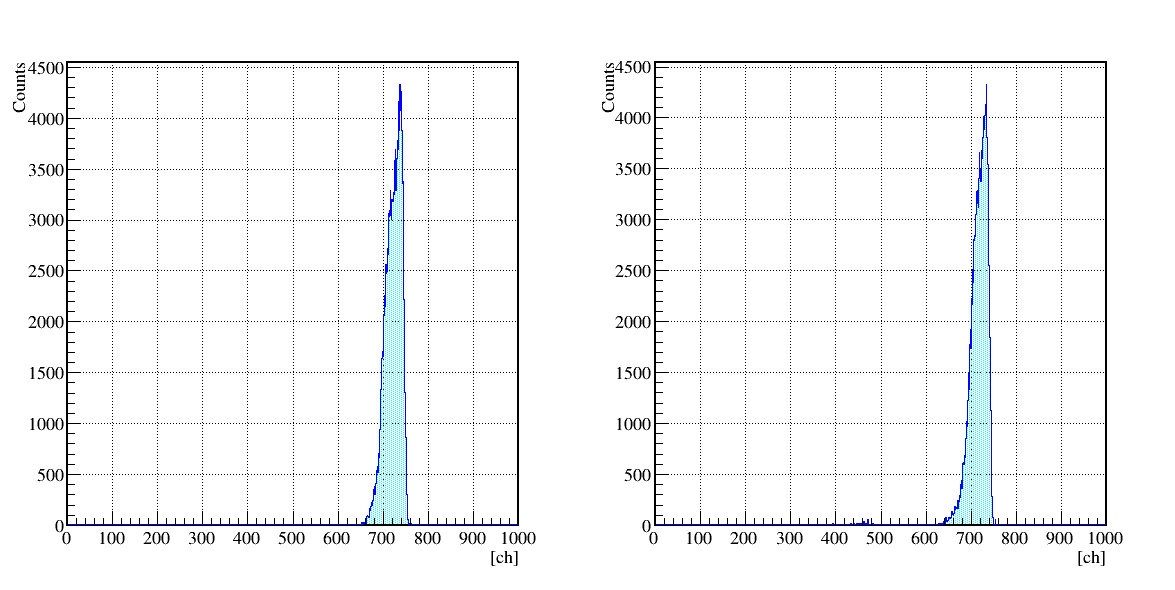
\includegraphics[width=14cm]{chapter4/tdc_bdcs.png}
    \caption{TDC Distribution of BDC1 (left) and BDC2 (right)}
    \label{TDC Distribution}
\end{figure}
Drift Chamber의 각 레이어에 검출된 위치 (x,y)를 통해 입자의 통과 궤적을 선형 fitting 으로 구할 수 있다. 이 궤적을 통해 각각의 layer에서의 위치가 Reconstruct된다.  STC (Space-Time Conversion) function 를 이용하여 각 layer에서의 위치와 시간을 통해 입자의 통과 궤적을 구할 수 있다. 
\begin{align}
    \frac{dN}{dx} = const.  
\end{align}
Then STC function is derived as follows.
\begin{align}
    \frac{dN}{dt} \cdot \frac{dt}{dx} &= const.\\
    dx &= C \cdot \frac{dN}{dt} \cdot dt,\\
    x(t) &= C \cdot \int_{t_{0}}^{t} \frac{dN}{dt} dt
\end{align}

\begin{align}
    \delta x = x_{calc} - x_{hit}
\end{align}
\subsection{Beam Profile at Target}
Target Chamber 주변에는 검출기가 없기 때문에 두개의 BDC를 이용하여 target에서의 Beam 위치를 외삽한다. 본 실험에서 사용하는 ${}^{17}B$는 본 실험의 main beam이 아니기 때문에, 위에서 확인한 BDC에서의 beam profile 과 같이 target 중심에서 ずれている。따라서 Target의 유효면적 x +/- 35mm, y +/- 35mm를 정의하고, 이를 넘어가는 이벤트는 제거한다.

\subsection{Beam beta calculation}
Invariant Mass를 계산하기 위해서는 Beam의 beta를 계산해야 한다. Beam의 beta는 다음과 같이 계산된다.

\subsubsection{Eloss Calculation}
Once $TOF_{F7-F13}$ has been calculated, the $\beta_{beam}$ can be calculated using the following equation. 

\begin{align}
    \beta_{F7-F13} = \frac{L(F7-F13)}{TOF_{F7-F13} \times c}
\end{align}

차후의 Invariant Mass 계산을 위해 target 중심에서의 beam-beta를 구할 필요가 있다. F5에서의 Brho를  beta는 tof713의 이차식으로 다음과 같이 나타낼 수 있다. 또한 각 특정 위치에 대한 coefficient는 표에 표시하였다.

\begin{align}
    TOF_{F7_Tgt} = a TOF_{F7-F13}^{2} + b TOF_{F7-F13} + c    \beta_{F5}  
\end{align}

\clearpage
\section{Analysis of charged fragment}
\subsection{FDC를 이용한 위치 계산}
\begin{table}
    \centering
    \begin{tabular}[h]{c|cc}
        \hline
        &$t_{min}$ [ch]&$t_{max}$ [ch]\\
        \hline
        FDC1&600&800\\
        FDC2&600&800\\        
        \hline
    \end{tabular}
    \caption[short]{TDC window condition of FDC1 and FDC2}
\end{table}
\begin{figure}
    \centering
    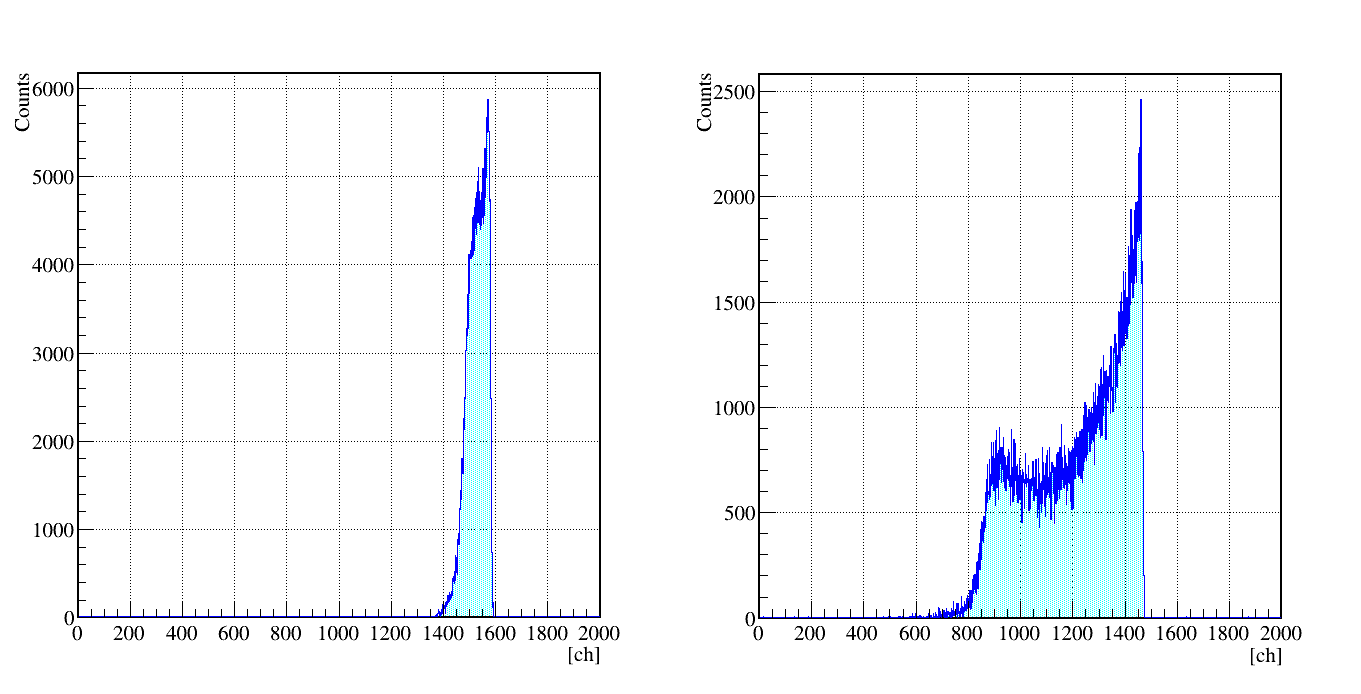
\includegraphics[width=14cm]{chapter4/tdc_fdcs.png}
    \caption{TDC Distribution of FDC1 (left) and FDC2 (right)}
    \label{TDC Distribution of FDCs}
\end{figure}
\subsection{Brho from Simulation}
\subsubsection{Simulation Using Monte Carlo Method}

\subsubsection{Numerical Calculation}
Optrace는 Magnetic Field 데이터를 기반으로 입자의 Transformation Matrix를 구하는 프로그램이다. 본 실험에서 사용된 SAMURAI의 profile은 3T의 중심자기장과 60도의 회전각도를 갖는다. 이를 기반으로 Optrace 자기장 파일을 작성한 결과, 자기장에 대한 Transformation Matrix는 다음과 같다.

\subsection{HODscope Z}
15B를 특정하기 위하여, Hodscope라는 Plastic Scintillator 검출기에서 Z를 특정한다.
상류에서 17B를 특정하여, 가장 많은 입자가 Z=5라고 가정, 위의 시뮬레이션으로 얻은 AOZ를 대입하여 15B를 특정한다.
\subsection{Fragment Particle Identification}
\begin{figure}
    \centering
    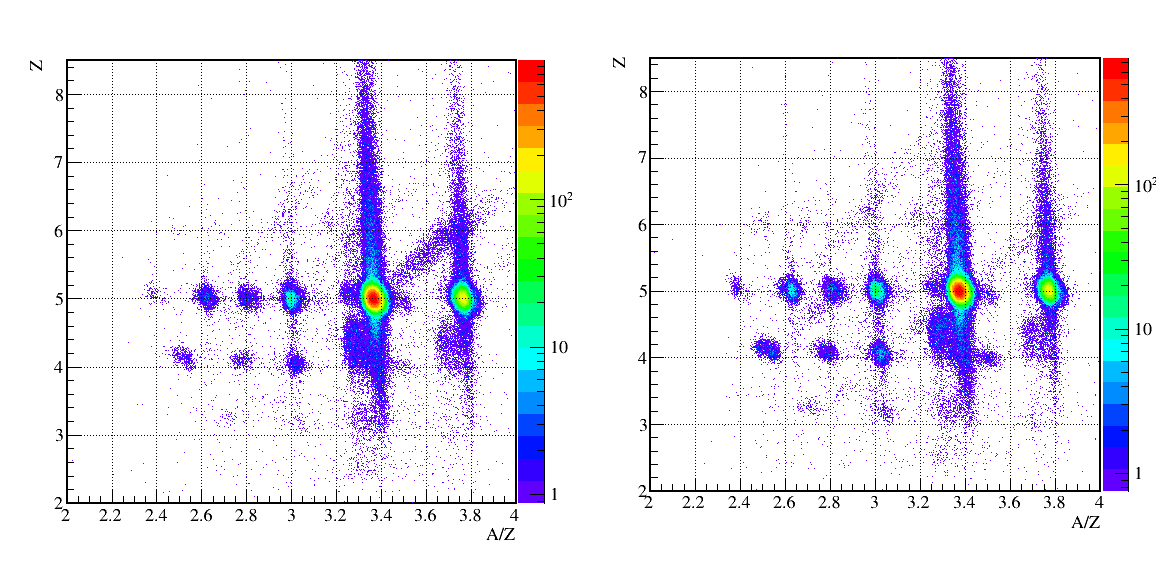
\includegraphics[width=14cm]{chapter4/fragpid_all.png}
    \caption{Fragment Particle Identification of All Events at Pb target (left) and C target (right)}
    \label{Fragment Particle Identification of All Events}
\end{figure}

\begin{figure}
    \centering
    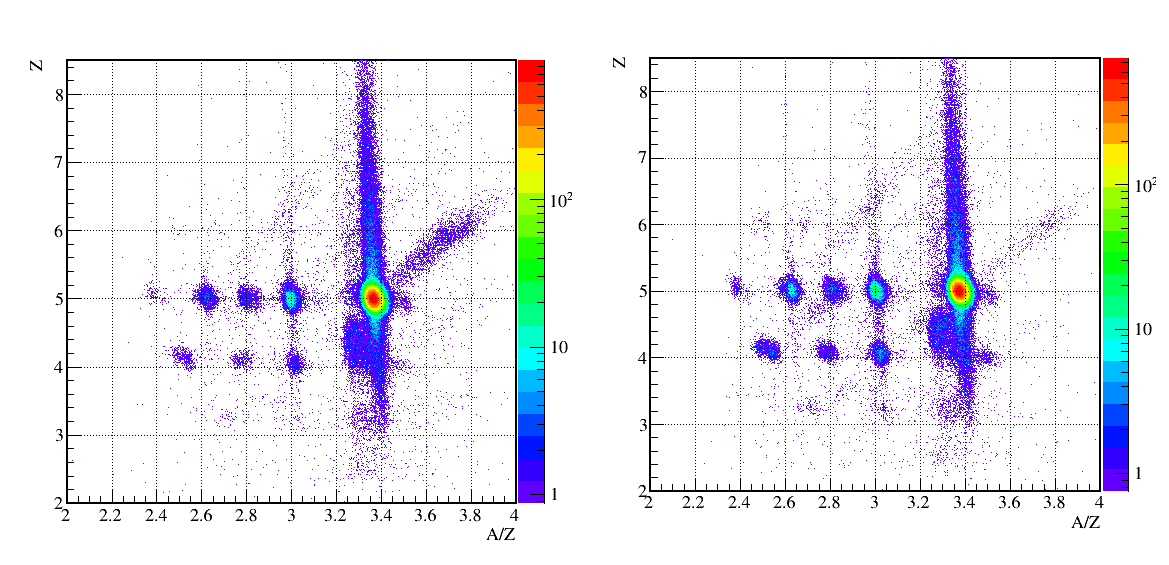
\includegraphics[width=14cm]{chapter4/fragpid_b17.png}
    \caption{Fragment Particle Identification of ${}^{17}$B Events at Pb target (left) and C target (right)}
    \label{Fragment Particle Identification of ${}^{17}$B Events}
\end{figure}

\clearpage

\section{Analysis of Neutrons}
A neutron is detected indirectly by recoiled charged particles which is mainly produced by H($n$,$n$) and ${}^{12}$C(n,np) reaction in the plastic-scintillator. \\
\indent In this experiment, neutrons emitted from the secondary beam ${}^{17}$B are detected by the NEBULA neutron detector system within the SAMURAI setup.  This section describes the process of selecting either single-neutron or two-neutron events using the NEBULA neutron detector array. The momentum $P(n)$ of the neutron is reconstructed from the detection position in NEBULA relative to the target, and the time-of-flight (TOF). The energy of the neutron is described as follows.
\begin{align}
    L &= | \vec{r}_{\text{tgt}} - \vec{r}_{n} | \\
    \beta_{n} &= L / (\text{TOF}_{\text{NEB-tgt}} \times c) \\
    P_{n} &= m_{n} \beta_{n} \gamma_{n} \\
    E_{n} &= m_{n} \gamma_{n} \\
    \vec{P_{n}} &= \frac{\vec{r_{n}} - \vec{r_{n}}}{L} P_{n}
\end{align}
where, $\vec{r}_{\text{tgt}}$ is the position of the target $\vec{r}_{\text{tgt}}$ = (), $m_{n}$ is the neutron mass ($m_n$ = MeV)

\subsection{Selection of Neutron Events}
Because of the indirect detection of neutrons, the selection of neutron events is more complicated than that of charged particles. The selection of neutron events is performed in four steps. First, reject the events which assumed as gamma event. Second, reject the events which is assumed as recoiled proton or gamma event. Third, in two neutron selection case, remove the event which is assumed as cross-talk. After all, select the fastest and second fastest event as a real neutron event. 

\subsubsection{gamma event rejection}
진짜 뉴트론 이벤트를 선택하기 위해서 감마선을 제거하는 스레숄드를 지정한다.
\begin{enumerate}
    \item 1st VETO에 hit한 이벤트는 모두 하전입자라 간주하여 제거한다.
    \item 중성자 검출기 NEBULA에 입사한 이벤트 중, 발광량 Q가 6MeVee 이하인 이벤트는 감마선으로 간주하여 제거한다. 또한 하나의 플라스틱 신틸레이터 모듈을 통과할 때의 중성자의 최대 에너지 loss 130MeV를 넘어가는 이벤트도 중성자에서 산란된 다른 이벤트로 간주하여 제거한다.
    \item Target에서부터의 TOF가 1st wall의 경우 40ns 이하, 2nd wall의 경우 42ns 이하인 이벤트 또한 중성자 이외의 이벤트로 간주하여 제거한다.
    \item (2중성자 이벤트에 대해서만) 2nd VETO에 hit한 이벤트에 대하여, 2nd NEUT wall에 입사한 가장 빠른 두 중성자 이벤트가 dr(xy)<500mm, 2ns <dt< 5ns 인 이벤트는 2nd VETO에서 기인한 cluster 산란 이벤트로 간주하여 제거한다.
\end{enumerate}

When selecting events of two neutrons, the most important process is the elimination of cross-talk. Cross-talk refers to the phenomenon where a single neutron generates multiple signals, which  Cross-talk is the most significant source of noise when selecting two-neutron events. \\
Cross-talk 제거에는 크게 3가지 단계가 있다. 
To reject cross-talk, a Geant4 simulation was performed to generate events of ${}^{16}\text{B} \to {}^{15}\text{B}+n$, thereby replicating cases where all two-neutron events are due to cross-talk. The details of the executed Geant4 simulation are as follows.
\begin{center}
    \begin{tabular}[h]{c|c}
        \hline \hline
        Reaction & ${}^{16}\text{B} \to {}^{15}\text{B}+n$ \\
        Beam Energy & 140 MeV/u\\
        Relative Energy & 0 - 10 MeV (Uniformly Generated)\\
        Position Distribution & Reconstructed from ${}^{17}$B Beam profile\\
        Angular Distribution & Reconstructed from ${}^{17}$B Beam profile \\
        \hline \hline
    \end{tabular}
\end{center}
\subsection{Clustering Event Subtraction}

\subsection{same wall event}
두 중성자

\subsubsection{cluster proton cross-talk}


\subsection{different wall}
\section{Cross-talk 잔존률 평가}
각각의 Cross talk 제거 단계에 따라 Cross-talk가 남아있는 비율을 평가하였다. 단계는 4단계로 나누어, 다음과 같이 구분한다. 
\begin{enumerate}
    \item (a) no rejection
    \item (b) clustering rejection
    \item (c) clustering rejection + same wall rejection
    \item (d) clustering rejection + same wall rejection + gamma rejection
\end{enumerate}
각 단계에서의 Cross-talk 잔존률은 다음과 같은 식으로 나타낸다. \
\begin{align}
    R = \frac{N_{M>2}}{N_{M>1}}
\end{align}
1n 시뮬레이션에서 잔존률 1$\%$를 목표로 분석을 진행하였다. 분석 결과 전체 M>1 event 225385 이며, 각 단계에서의 M>2 event와 잔존률 R은 다음과 같다. 조건 d까지 적용하였을 때 각각의 Wall에서 잔존률이 1$\%$ 이하로 낮아지는 것을 확인할 수 있다.
\begin{center}
    \begin{tabular}[h]{c|c|c|c}
        \hline
        Condition & same wall event (R) & different wall event (R) & all wall event (R)\\
        \hline
        (a) & 89721 (39.8$\%$) & 10123 (4.5$\%$) & 99844 (44.3$\%$) \\
        (b) & 29032 (12.9$\%$) & 16848 (7.5$\%$) & 45880 (20.4$\%$)\\
        (c) & 6274 (2.8)$\%$)   & 2791 (1.2$\%$)& 9065 (4.0$\%$)\\
        (d) & 5352 (2.4$\%$)& 2089 (0.9$\%$)& 7441 (3.3$\%$)\\
        \hline
    \end{tabular}
\end{center}

\section{Acceptance and Efficiency Correction}
SAMURAI의 Acceptance and Efficiency를 평가하기 위해 Geant4 Simulation을 진행했다. 시뮬레이션 정보는 다음과 같다 
\begin{center}
    \begin{tabular}[h]{c|c}
        \hline
        Physics Model & Phase Space Decay \\
        
        Beam Energy & 270 MeV/u\\
        Relative Energy & 1-10 MeV (Uniformly generated)\\
        \hline
    \end{tabular}
\end{center}

\begin{figure}
    \centering
    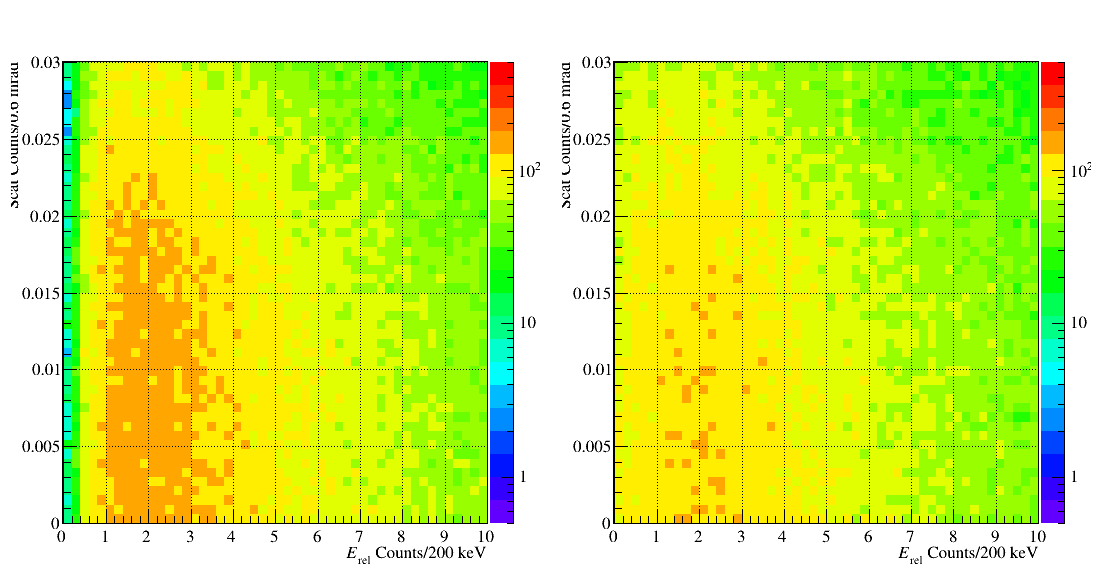
\includegraphics[width=14cm]{chapter4/acc_same_diff.png}
    \caption{2n Acceptance for same wall (left) and different wall (right)}
    \label{2n Acceptance for same wall (left) and different wall (right)}
\end{figure}




\section{Experimental Resolution}


\section{Relative Energy Spectrum}
\begin{figure}
    \centering
    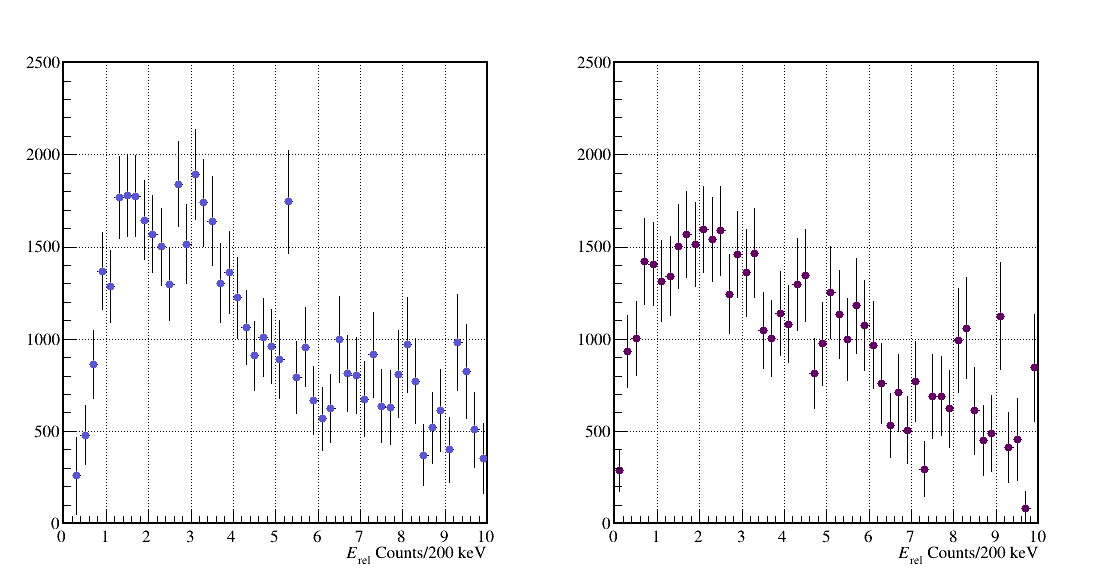
\includegraphics[width=14cm]{chapter4/Pb_same_diff.png}
    \caption{Relative Energy Spectrum of Pb target}
    \label{Relative Energy Spectrum of Pb target}
\end{figure}
\begin{figure}
    \centering
    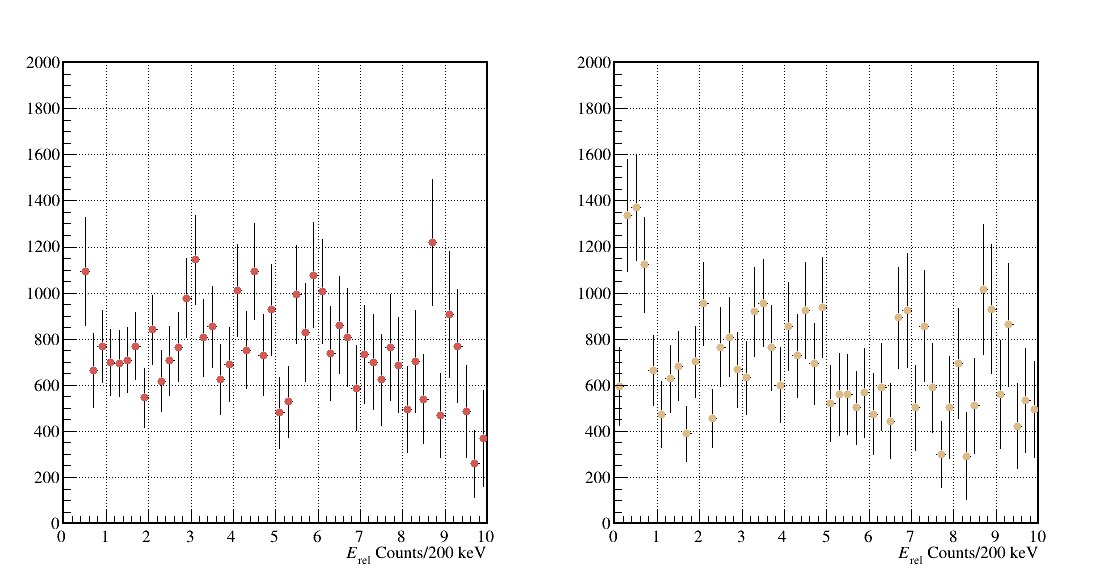
\includegraphics[width=14cm]{chapter4/C_same_diff.png}
    \caption{Relative Energy Spectrum of C target}
    \label{Relative Energy Spectrum of C target}
\end{figure}

\begin{figure}
    \centering
    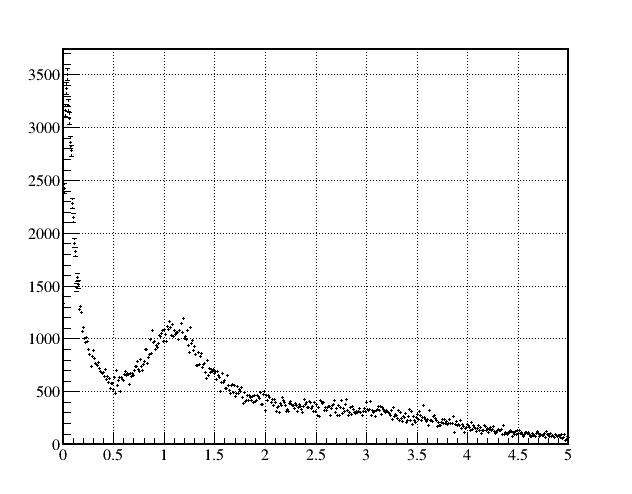
\includegraphics[width=14cm]{chapter4/16Bn_C.png}
    \caption{Relative Energy Spectrum of ${}^{16}$B + n at C target}
    \label{Relative Energy Spectrum of ${}^{16}$B + n C target}
\end{figure}



\section{Exclusive Cross Section}   